\documentclass{standalone}

\usepackage{tikz}
\usetikzlibrary{arrows,automata}
\usepackage{xcolor}
\definecolor{myblue}{RGB}{0,0,127} % navy blue


\begin{document}
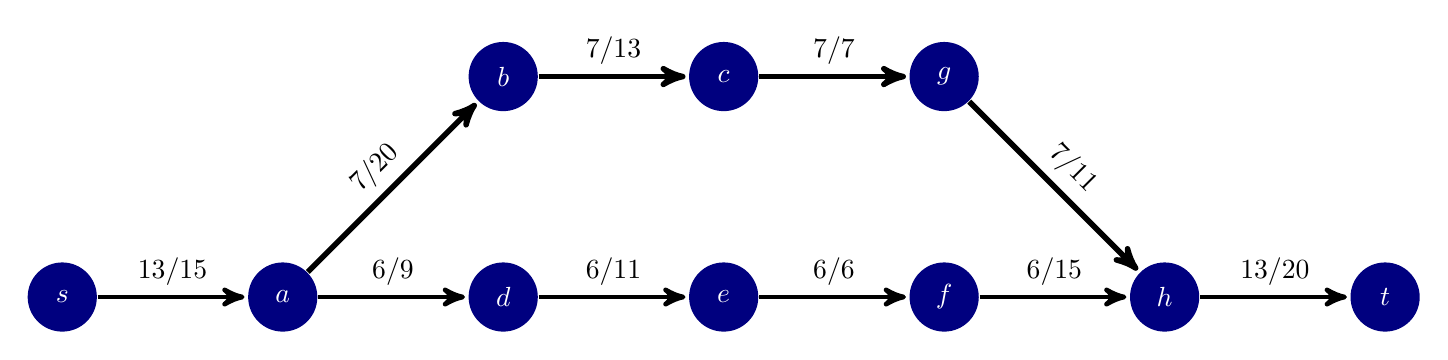
\begin{tikzpicture}[->,>=stealth',shorten >=1pt,auto,node distance=2.8cm, semithick]
  \tikzstyle{every state}=[fill=myblue,draw=none,text=white]

  \node[state]         (S)              {$s$};
  \node[state]         (A) [right of=S] {$a$};
  \node[state]         (B) [right of=S, above of=A] {$b$};
  \node[state]         (C) [right of=B] {$c$};
  \node[state]         (D) [below of=B] {$d$};
  \node[state]         (E) [right of=D] {$e$};
  \node[state]         (F) [right of=E] {$f$};
  \node[state]         (G) [right of=C] {$g$};
  \node[state]         (H) [right of=F] {$h$};
  \node[state]         (T) [right of=H] {$t$};

  \path[line width=0.7mm]
        (A) edge  node[sloped, anchor=center,above] {$7/20$}  (B)
        (B) edge  node[sloped, anchor=center,above] {$7/13$}  (C)
        (C) edge  node[sloped, anchor=center,above] {$7/7$}  (G)
        (G) edge  node[sloped, anchor=center,above] {$7/11$}  (H);
  \path[line width=0.6mm] 
        (S) edge  node[sloped, anchor=center,above] {$13/15$}  (A)
        (A) edge  node[sloped, anchor=center,above] {$6/9$}  (D)
        (D) edge  node[sloped, anchor=center,above] {$6/11$}  (E)
        (E) edge  node[sloped, anchor=center,above] {$6/6$}  (F)
        (F) edge  node[sloped, anchor=center,above] {$6/15$}  (H)
        (H) edge  node[sloped, anchor=center,above] {$13/20$}  (T);
\end{tikzpicture}
\end{document}
